\documentclass[a4paper,12pt]{article}

\usepackage{graphicx}
\usepackage[brazilian]{babel}
\usepackage[utf8]{inputenc}
\usepackage{fancyhdr}

\pagestyle{fancy}

\renewcommand{\headrulewidth}{0.0pt}
\renewcommand{\footrulewidth}{0.0pt}
\fancyhead{}
\fancyhead[CO,CE]{versão 0.15}

\def\cms{\emph{CMS}}
\def\rss{\emph{RSS}}
\def\plugin{\emph{plugin}}

\begin{document}

\title{Software para integração de \emph{feeds} e sistemas de gerenciamento de conteúdo}
\author{Marcelo Toledo \and Rafael Castilho}
\date{\today}
\maketitle

\newpage
\section{Introdução}

\paragraph{}
Sistemas de gerenciamento de conteúdo (\cms{}), em particular os populares \emph{blogs}, são ferramentas que permitem a publicação de conteúdo em um endereço \emph{WEB}, e que exigem apenas o conhecimento do uso da \emph{interface}.
\paragraph{}
Em geral, os \cms{}s permitem a visualização de itens de conteúdo publicado na forma parametrizada \rss{} por meio de canais alimentadores (\emph{feeds}). Uma das ferramentas mais utilizadas pelos \emph{blogueiros} é o agregador de \rss{}, capaz de coletar e organizar o conteúdo de diversos canais simultaneamente.
\paragraph{}
Em um \emph{blog}, além de conteúdo próprio, é comum a citação de conteúdo de terceiros, realizado de forma "artesanal", através da cópia das informações disponíveis na página \emph{WEB} ou no agregador e da colagem no editor de publicação do \cms{}.
\paragraph{}
O objetivo do software a ser desenvolvido é disponibilizar um agregador de canais que permita a publicação de itens de conteúdo no \cms{} do cliente de forma ágil, padronizada, e com base em suas preferências.

\section{Especificação funcional}

\subsection{Autenticação e cadastro de perfil de acesso}

\paragraph{}
Para ter acesso ao software, o cliente deve efetuar a autenticação de um perfil de acesso a partir de um endereço de e-mail e senha cadastrados.
\paragraph{}
O cadastro de um novo perfil de acesso é feito a partir do formulário de autenticação, através da opção "não cadastrado", que quando acionada, passa a exibir o formulário para um novo cadastro. 
\paragraph{}
\begin{center}
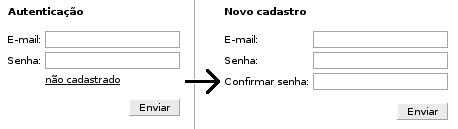
\includegraphics[scale=0.8]{authform.png}
\end{center}
\paragraph{}
O procedimento para criação de um novo perfil a partir do formulário para um novo cadastro deve ser feito como segue:
\begin{itemize}
\item Informar um endereço de e-mail, senha e confirmação de senha;
\item Se o endereço de e-mail não estiver cadastrado em um perfil de acesso, o cliente deverá receber uma mensagem de e-mail contendo uma \emph{URL} de confirmação de cadastro;
\item Após a confirmação de cadastro, o cliente deverá reber uma mensagem de e-mail contendo uma notificação de cadastro confirmado, boas vindas e instruções para o primeiro acesso.
\item Se o endereço de e-mail informado já estiver cadastrado, o cliente deverá receber uma mensagem de e-mail contendo uma notificação da existência do perfil com instruções para acesso e alteração de senha (se necessário).
\end{itemize}
\paragraph{}
Em uma situação onde o cliente afirme já possuir um perfil de acesso mas não lembra-se da senha, o software deve permitir a recuperação do acesso, através da seguinte forma:
\begin{itemize}
\item Informar o endereço de e-mail do perfil de acesso;
\item Se o endereço de e-mail estiver cadastrado em um perfil de acesso, o cliente receberá uma mensagem de e-mail com uma \emph{URL} para o formulário de alteração de senha;
\item O formulário de alteração de senha permite ao cliente digitar uma nova senha. Após a alteração, o software deverá enviar uma mensagem de e-mail ao cliente com a notificação de alteração.
\item Se o endereço de e-mail informado não estiver associado a um perfil de acesso, o cliente deverá receber uma mensagem de e-mail com a notificação da não existência do perfil de acesso e instruções para a criação de um novo.
\end{itemize}
\paragraph{}
Após efetuar o acesso, o cliente poderá alterar sua senha e preencher as informações pessoais em seu perfil:

\begin{itemize}
\item Nome;
\item País;
\item Região;
\item Cidade;
\item Distrito;
\item Endereço;
\item Código postal
\end{itemize}

\subsection{Cadastro de \cms{}}

\paragraph{}
Após efetuar acesso, o cliente poderá realizar o cadastro de um novo \cms{} através das seguintes etapas:

\begin{itemize}
\item Informar a \emph{URL} raiz do \cms{}. O software deverá detectar o tipo de \cms{} (\emph{Wordpress}, \emph{Joomla}, \emph{Drupal}, etc.) a partir da \emph{URL} informada;
\item Se for possível a detecção do tipo de \cms{}, o software deverá verificar a existência do gerenciador de publicações do \cms{} em um endereço padrão, de acordo com o tipo de \cms{} e da \emph{URL} raiz;
\item Se o gerenciador de publicações do \cms{} não estiver disponível no endereço padrão, permitir que o cliente informe seu endereço através de uma \emph{URL}. O software deverá verificar se o endereço informado é válido como gerenciador de publicações para o tipo de \cms{} escolhido;
\item Se a detecção do tipo de \cms{} não for bem sucedida, verificar a causa e informar o erro mais provável (endereço ou página não encontrados, erro no servidor, etc.);
\item Se o endereço estiver correto mas o tipo não for suportado, exibir notificação ao cliente e informar os tipos suportados. Permitir também que o cliente digite o tipo utilizado. Neste caso, o cadastro de \cms{} não poderá prosseguir;
\item Após a determinação precisa do tipo de \cms{} e endereço do gerenciador de publicações, solicitar ao cliente que informe o usuário e senha do gerenciador. O software deverá verificar se o usuário e senha permitem acesso ao gerenciador, caso contrário, notificar que o usuário e senha não são válidos;
\item O software deve verificar de forma não invasiva (sem publicar conteúdo em produção) se o acesso ao gerenciador de publicações possui permissão para escrita de conteúdo (ex. \emph{drafts} do \emph{Wordpress}). Se não for possível tal verificação, o software poderá solicitar ao cliente se deseja realizar um teste de publicação em produção.
%\item Tipo de \cms{} (\emph{Wordpress}, \emph{Joomla}, \emph{Drupal}, etc.);
% \item Endereço do gerenciador de publicações do \cms{};
% \item Usuário e Senha do gerenciador de publicações do \cms{};
\item Recursos a serem utilizados;
\item Método de publicação;
\end{itemize}

\subsubsection{Tipo de \cms{}}

...o plugin deve gerenciar diferenças de versão...

\paragraph{}
Os tipos de \cms{} disponíveis para o cliente serão adicionados ao software no formato de \emph{plugins}, e devem seguir um protocolo de comunicação com o software.

\subsubsection{Recursos}

\paragraph{}
O protocolo determinará quais recursos estarão disponíveis no software e que poderão ser utilizados pelo \plugin{}. O \plugin{} determina a implementação do recurso de acordo com o \cms{}.
\paragraph{}
O protocolo de comunicação deve estabelecer os recursos mínimos para o funcionamento do software, e que serão de implementação obrigatória para um \plugin{}, dos quais:

\begin{itemize}
\item Publicação de item contendo título, descrição e comentários;
\end{itemize}

\paragraph{}
Outros recursos adicionais também poderão ser incluído ao protocolo quando forem necessários.

\paragraph{}
As opções de escolha na utilização de recursos é determinado pelo tipo de \cms{} escolhido. No entanto os recursos obrigatórios definidos pelo protocolo são utilizados por padrão e não permitem alterações.

\subsubsection{Método de publicação}

\paragraph{}
A publicação de conteúdo em um \cms{} deve ser feita de forma manual, a partir dos itens de conteúdo disponibilizados pelos canais. No entanto é possível automatizar este processo, a partir da configuração dos seguintes filtros:

\begin{itemize}
\item Alimentação: Define a lista de canais a serem utilizados. Padrão: Todos os cadastrados;
\item Ordenação: Define a ordem de publicação a partir da data de publicação, popularidade ou randômico. Padrão: Data de publicação;
\item Frequência: Define o intervalo de tempo entre as publicações. Mínimo: 5 minutos;
\item Palavras-chave: A escolha de itens é feita com base em uma ou mais palavras-chave;
\item Com estrela: Somente itens de conteúdo marcados com estrela serão utilizados para publicação;
\end{itemize}

\paragraph{}
Independentemente da configuração estabelecida para a publicação automática, a opção manual deverá sempre estar disponível.

\paragraph{}
A popularidade pode ser medida através da quantidade de publicações feitas por outros clientees para um mesmo item.

\subsection{Cadastro de canais \rss{}}

\paragraph{}
O software deve permitir a inclusão de canais a partir da \emph{URL} do alimentador ou da importação de arquivos \emph{OPML}.
\paragraph{}
A atualização dos itens de conteúdo dos canais serão gerenciados pelo sistema de armazenamento de conteúdo.
\paragraph{}

\subsubsection{Sistema de armazenamento de conteúdo}

\paragraph{}
Os itens de conteúdo de um canal podem ser globais, ou seja, podem ser compartilhados por todos os clientees do software, afim de eliminar redundância desnecessária de dados.
\paragraph{}
Quando um novo canal é adicionado, o sistema se preocupa em obter os itens mais recentes deste canal imediatamente.
\paragraph{}
Para um canal já existente, o sistema deverá executar em \emph{background} e obter novos itens, com uma freqüência que depende da freqüencia de publicação de conteúdo neste canal.

\subsection{Área de trabalho}

\paragraph{}
Durante a sessão de um perfil, o software deverá exibir a área de trabalho, contendo painéis com a listagem de canais \rss{} e \cms{} cadastrados.
\paragraph{}
Em um painel central, serão exibidos os itens disponíveis de todos os canais \rss{} cadastrados no perfil. Ao selecionar um canal, o painel deverá exibir apenas os itens do canal selecionado.

\subsubsection{Painel central}

\paragraph{}
O cliente poderá determinar a quantidade de itens de conteúdo que devem aparecer no painel central, de acordo com as suas preferências.
\paragraph{}
A ordem de visualização dos itens é por padrão em ordem decrescente da data de publicação, mas também poderá ser ordenado pela popularidade ou de forma randômica.
\paragraph{}
Um item poderá ser marcado com uma estrela, permitindo que seja facilmente encontrado posteriormente.
\paragraph{}
Um item de conteúdo poderá ser "arrastado" para um item do painel de \cms{}. Em seguida, uma janela de publicação será exibida, onde o cliente deverá acionar o botão "enviar" para publicar o conteúdo no \cms{}.

\subsubsection{Janela de publicação}
\paragraph{}
A janela de publicação deve conter o título e descrição do item de conteúdo, além de um campo para adicionar comentários. A janela deve permitira a edição dos valores iniciais.
\paragraph{}
Outros recursos podem estar disponíveis conforme o \cms{} utilizado.

\section{Notas}

\paragraph{}
Quando um tipo de \cms{} não for suportado, e o cliente informar o tipo de \cms{} utilizado, o \emph{backend} poderá verificar se houve falha na detecção e solicitar ajuste no desenvolvimento, e informar ao cliente sobre a resolução do problema. Se o tipo não for suportado, informar ao cliente que o software não é suportado. É possível também verificar quais são as tendências para implementações de novos tipos.
\paragraph{}
O software deverá servir como guia para padronização da publicação de conteúdo externo, com a virtude de previnir ao cliente problemas com \emph{copyright}, por exemplo.

\subsection{Segurança}

\paragraph{}
O software deve limitar a quantidade de mensagens de e-mail enviadas durante a solicitação de um novo cadastro de perfil ou durante a recuperação de acesso a um perfil de acesso, afim de evitar uso mal intencionado do envio de mensagens.
\paragraph{}
O software deve conter algum tipo de proteção para que as publicações em um \cms{} não sejam feitas por seu próprio alimentador automaticamente e indefinidamente (autófago).

\end{document}
